\openepigraph{Memory... is the diary that we all carry about with us.}{---Oscar Wilde}

\section{How to write a research report}

Bean, J. C. (2001). Engaging ideas: The professor’s guide to integrating writing, critical thinking, and active learning in the classroom. San Francisco: Jossey-Bass Publishers

A formal scientific research report is a piece of professional writing addressed to other professionals who are interested in the investigation you conducted. They will want to know why you did the investigation, how you did it, what you found out, and whether your findings were significant and useful. Research reports usually follow a standard five-part format: (1) introduction, (2) methods, (3) results (4) discussion of results, and (5) conclusions and recommendations.

\subsection{Introduction} 
Here you explain briefly the purpose of your investigation. What problem did you address? Why did you address it? You will need to provide enough background to enable the reader to understand the problem being investigated. Sometimes the introduction also includes a “literature review” summarizing previous research addressing the same or a related problem. In many scientific disciplines, it is also conventional to present a hypothesis—a tentative “answer” to the question that your investigation will confirm or disconfirm.

\subsection{Methods} 
This is a “cookbook” section detailing how you did your investigation. It provides enough details so that other researchers could replicate your investigation. Usually, this section includes the following subsections: (a) research design, (b) apparatus and materials, and (c) procedures followed.

\subsection{Results} 
This section sometimes headed “Findings,” presents the empirical results of your investigation. Often, your findings are displayed in figures, tables, graphs, or charts that are referenced in the text. Even though the data are displayed in visuals, the text itself should also describe the most significant data. (Imagine that the figures are displayed on a view graph and that you are explaining them orally, using a pointer. Your written text should transcribe what you would say orally.) Your figures and tables must have sufficient information to stand along, including accurate titles and clear labels for all meaning-carrying features.

\subsection{Discussion of results} 
This is the main part of the report, the part that will be read with the most care by other professionals. Here you explain the significance of your findings by relating what you discovered to the problem you set out to investigate in your introduction. Did your investigation accomplish your purpose? Did it answer your questions? Did it confirm or disconfirm your hypothesis? Are you results useful? Why or why not? Did you discover information that you hadn’t anticipated? Was your research design appropriate? Did your investigation raise new questions? Are there implications from your results that need to be explored? The key to success in this section is to link your findings to the questions and problems raised in the introduction.

\subsection{Conclusions and recommendations} 
In this last section, you focus on the main things you learned from the investigation and, in some cases, on the practical applications of your investigation. If your investigation was a pure research project, this section can be a summary of your most important findings along with recommendations for further research. If your investigation was aimed at making a practical decision (for example, an engineering design decisions), here you recommend appropriate actions. What you say in this section depends on the context of your investigation and the expectations of your readers.

\section{APA style}

The next sections provide information about APA style, and an example research report written in APA style.

\subsection{APA style formatting}

\includepdf[pages=1-6]{APA1.pdf}

\subsection{Sample APA report}

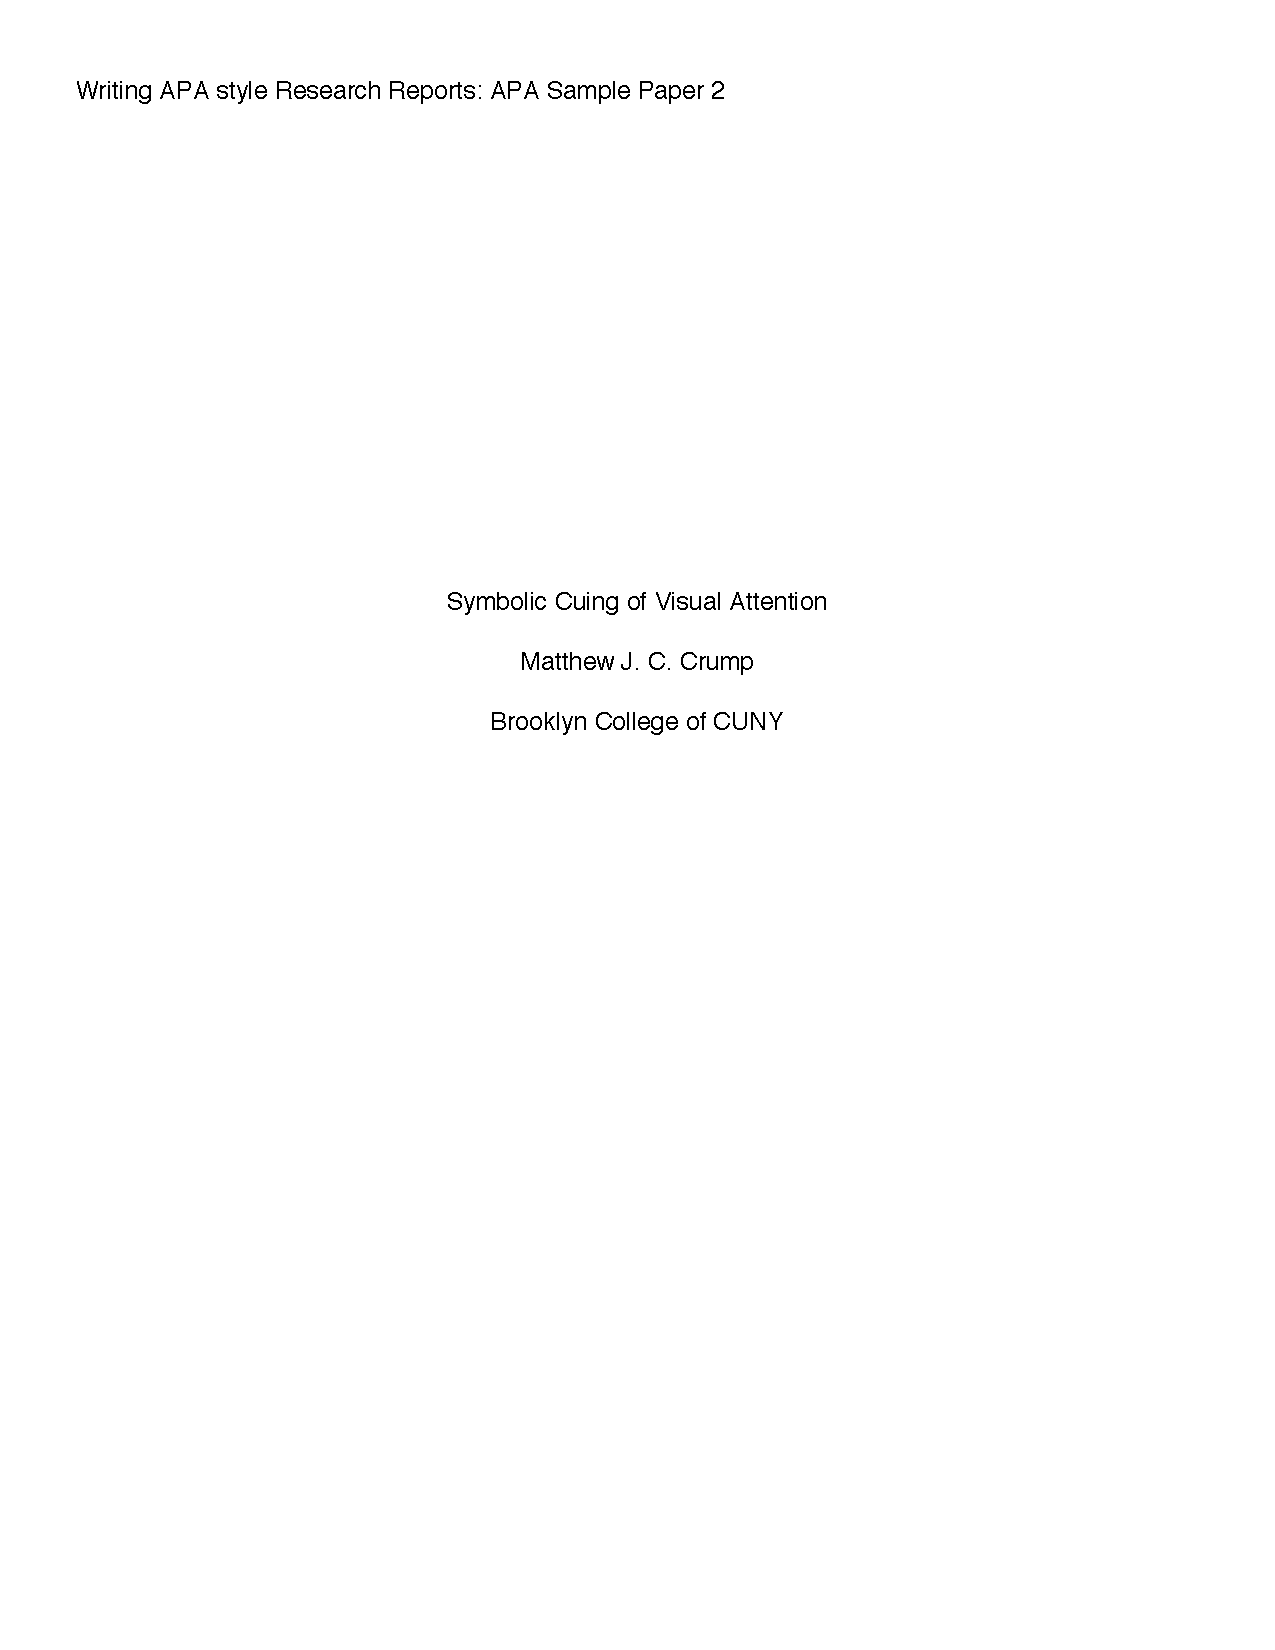
\includepdf[pages=1-8]{APA2.pdf}

